\subsubsection{Constructing the predicate tree}
\label{sec:Construct}
Every predicate in the \textit{fuzzy program} $P_{new}$ could be represented as a tree. A formal description of the approach of generating a corresponding tree for a certain predicate begins with the definition of \textit{atomic predicate} and \textit{complex predicate}.
 
\begin{defin}\textbf{(Atomic predicate)}.
Predicates appearing only in the bodies of rules in $R_{new}$, and never appearing in the heads of any rules, are \textbf{atomic predicates}, since they are not defined by any other predicates.  
\end{defin}

\begin{defin}\textbf{(Complex predicate)}.
Predicates appearing in the heads of rules in $R_{new}$ are \textbf{complex predicates}, in the sense that they could be represented by the bodies of the rules with them as heads. 
\end{defin}

\textit{Atomic predicate} is written as $p_{a}$, and \textit{complex predicate} as $p_{c}$. \textit{Atomic predicate} $p_{a}$ is represented in a tree-form, which is a node with information $\tau_{p_{a}}$, and without any children nodes, where $\tau_{p_{a}}$ is the \textit{type} of $p_{a}$. \textit{Complex predicate} $p_{c}$ by definition must appear in the head of some rules in $P_{new}$, whose form is,
\[p_{c}(\vec{t}) \stackrel{c,F_c}{\longleftarrow}F(p_1(\vec{t_1}),...,p_n(\vec{t_n}))\] 
Then the tree of $p_{c}$ has a root $N_{p_{c}}$, with its node information, $c$, $F_c$, $F$, and $\tau_{p_{c}}$, which is the \textit{type} of $p_{c}$. The branches from $N_{p_{c}}$ are $N_{p_1}$, ..., $N_{p_n}$, which are expanded as corresponding trees recursively. Thus, the leaves in the tree are \textit{atomic predicates}, which never appear in the heads of any rules in $R_{new}$, and can not be expanded any more.

If there are several rules defining a certain predicate $p$, then there are different corresponding trees for $p$, since the expanding procedure is recursive, which means, the children of $p$ node could also be defined in several other rules, then more possible trees are generated. 

%\newpage
\begin{figure}[t]
\begin{center}
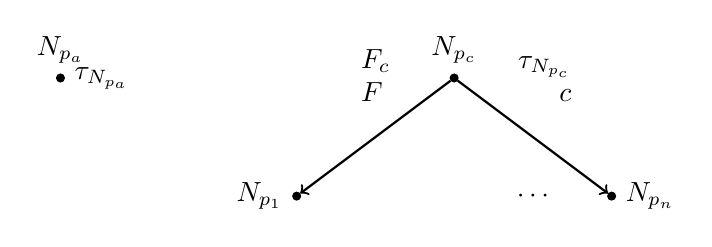
\begin{tikzpicture}[yscale=-1,
place/.style={circle,draw=black, fill=black, inner sep=0pt, 
              minimum size=1mm}]

 \node[place] (1st) at (1, 0) [label=above: $N_{p_{a}}$,
                               label=right: $\tau_{N_{p_{a}}}$] {};
	

\begin{scope}[xshift=4cm]
  \node[place] (1st) at (2, 0) [label=above: $N_{p_{c}}$,
                                label=right: 
       \begin{tabular}{l r}
         & $\tau_{N_{p_{c}}}$ \\
         & $c$\\
       \end{tabular},
       label=left:
       \begin{tabular}{l l}
         $F_c$ &\\
         $F$ &\\
       \end{tabular}] {};
  \node[place] (2nd) at (0, 1.5) [label=left: $N_{p_1}$] {};
  \node[place] (3rd) at (4, 1.5) [label=right: $N_{p_n}$]{}; 

  \node (dots) at (3,1.5) {$\cdots$};
	
  \draw[->, thick] (1st) -- (2nd);
  \draw[->, thick] (1st) -- (3rd);
\end{scope}

\end{tikzpicture}
\caption{Predicate Tree}
\label{Predicate Tree}
\end{center}   
\end{figure}

% pictures

\begin{ex}\label{ConstructPredicateTree}
Here is a part of short RFuzzy program,
\begin{center}
\begin{tabular}{l l}
$has\_tasty\_food:$  & $(Restaurant)$\\

$has\_healthy\_food:$ &  $(Restaurant)$\\

$has\_good\_service:$  & $(Restaurant)$\\

$tasty\_restaurant:$  & $(Restaurant)$\\

$good\_restaurant:$  & $(Restaurant)$\\
\end{tabular}
\end{center}
\begin{tabular}{l l l}
$tasty\_restaurant(X)$ & $\stackrel{1.0,.}{\longleftarrow} prod$ & $has\_tasty\_food(X)$\\

$good\_restaurant(X)$ & $\stackrel{0.8,.}{\longleftarrow} prod$ & $has\_healthy\_food(X), has\_good\_service(X)$ \\

\end{tabular}
\[Sim(has\_healthy\_food, has\_tasty\_food) = 0.6\]
\end{ex}

The corresponding trees for atomic predicates $has\_tasty\_food$,
$has\_healthy\_food$, \linebreak[4] $has\_good\_service$ are,
\begin{center}
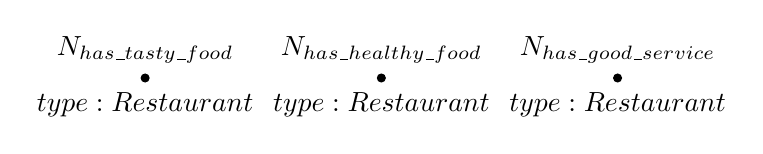
\begin{tikzpicture}[yscale=-1,
place/.style={circle,draw=black, fill=black, inner sep=0pt, 
              minimum size=1mm}]

 \node[place] (1st) at (0, 0) [label=above: $N_{has\_tasty\_food}$,
                               label=below: $type : Restaurant$] {};
	

\begin{scope}[xshift=3cm]
  \node[place] (1st) at (0, 0) [label=above: $N_{has\_healthy\_food}$,
                               label=below: $type : Restaurant$] {};
\end{scope}

\begin{scope}[xshift=6cm]
  \node[place] (1st) at (0, 0) [label=above: $N_{has\_good\_service}$,
                               label=below: $type : Restaurant$] {};
\end{scope}

\end{tikzpicture}
\end{center}   
The corresponding tree for complex predicate $tasty\_restaurant$ is,
\begin{center}
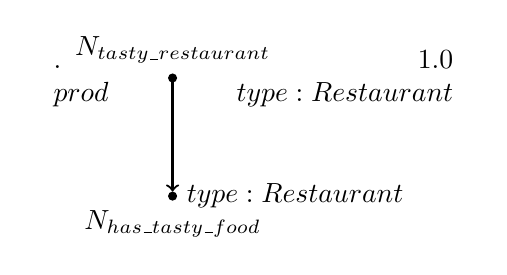
\begin{tikzpicture}[yscale=-1,
place/.style={circle,draw=black, fill=black, inner sep=0pt, 
              minimum size=1mm}]

 \node[place] (1st) at (0, 0) [label=above: $N_{tasty\_restaurant}$,
                                label=right: 
       \begin{tabular}{l r}
         & $1.0$\\
         & $type : Restaurant$ \\
       \end{tabular},
       label=left:
       \begin{tabular}{l l}
         $.$ &\\
         $prod$ &\\
       \end{tabular}] {};
  \node[place] (2nd) at (0, 1.5) [label=below: $N_{has\_tasty\_food}$,
                                  label=right: $type : Restaurant$] {};
 
  \draw[->, thick] (1st) -- (2nd);

\end{tikzpicture}
\end{center}   
The corresponding tree for complex predicate $good\_restaurant$ is,
\begin{center}
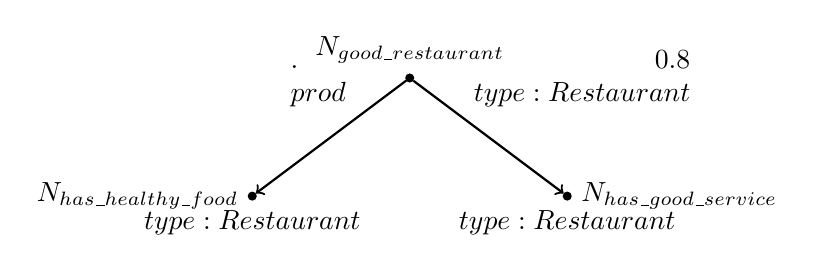
\begin{tikzpicture}[yscale=-1,
place/.style={circle,draw=black, fill=black, inner sep=0pt, 
              minimum size=1mm}]

  \node[place] (1st) at (2, 0) [label=above: $N_{good\_restaurant}$,
                                label=right: 
       \begin{tabular}{l r}
         & $0.8$\\
         & $type : Restaurant$ \\
       \end{tabular},
       label=left:
       \begin{tabular}{l l}
         $.$ &\\
         $prod$ &\\
       \end{tabular}] {};
  \node[place] (2nd) at (0, 1.5) [label=left: $N_{has\_healthy\_food}$,
                                  label=below: $type : Restaurant$] {};
  \node[place] (3rd) at (4, 1.5) [label=right: $N_{has\_good\_service}$,
                                  label=below: $type : Restaurant$]{}; 

  \draw[->, thick] (1st) -- (2nd);
  \draw[->, thick] (1st) -- (3rd);

\end{tikzpicture}
\end{center}   


\begin{comment}
\begin{prop} \textbf{Number of corresponding tree for predicate $p$}
The number of the corresponding trees for each predicate is exponential over the number of rules $n$.
\end{prop}

Let $P$ be a RFuzzy program, it has rules in the following form,
\[p() :- p_1(\vec{X})\]
\[p_1(\vec{X}) :- p_{11}(\vec{X})\]
\[p_1(\vec{X}) :- p_{12}(\vec{X})\]
\[p_{11}(\vec{X}) :- p_{111}(\vec{X})\]
\[p_{11}(\vec{X}) :- p_{112}(\vec{X})\]
\[p_{12}(\vec{X}) :- p_{121}(\vec{X})\]
\[p_{12}(\vec{X}) :- p_{122}(\vec{X})\]
\[\vdots\]
continue, for each predicate $p_{i}$, there are two rules defining it, in each rule, there is only one atom in the body.

Suppose that there is $n$ rules in $P$, and the number of trees could be generated for predicate $p$ is $2^{n/2}$, which is exponential of n. However, practically, the number of corresponding trees for certain predicate will not achieve the exponential, since the rules will be defined more reasonable, rather than the given example.

In order to retrieve the similarity between two predicates, creating all their corresponding trees is not optimal approach, considering the possible exponential explosion.  Therefore, there is a more efficient algorithm is proposed in the following sections.  

\end{comment}